% Options for packages loaded elsewhere
\PassOptionsToPackage{unicode}{hyperref}
\PassOptionsToPackage{hyphens}{url}
\PassOptionsToPackage{dvipsnames,svgnames,x11names}{xcolor}
%
\documentclass[
  letterpaper,
  DIV=11,
  numbers=noendperiod]{scrartcl}

\usepackage{amsmath,amssymb}
\usepackage{iftex}
\ifPDFTeX
  \usepackage[T1]{fontenc}
  \usepackage[utf8]{inputenc}
  \usepackage{textcomp} % provide euro and other symbols
\else % if luatex or xetex
  \usepackage{unicode-math}
  \defaultfontfeatures{Scale=MatchLowercase}
  \defaultfontfeatures[\rmfamily]{Ligatures=TeX,Scale=1}
\fi
\usepackage{lmodern}
\ifPDFTeX\else  
    % xetex/luatex font selection
\fi
% Use upquote if available, for straight quotes in verbatim environments
\IfFileExists{upquote.sty}{\usepackage{upquote}}{}
\IfFileExists{microtype.sty}{% use microtype if available
  \usepackage[]{microtype}
  \UseMicrotypeSet[protrusion]{basicmath} % disable protrusion for tt fonts
}{}
\makeatletter
\@ifundefined{KOMAClassName}{% if non-KOMA class
  \IfFileExists{parskip.sty}{%
    \usepackage{parskip}
  }{% else
    \setlength{\parindent}{0pt}
    \setlength{\parskip}{6pt plus 2pt minus 1pt}}
}{% if KOMA class
  \KOMAoptions{parskip=half}}
\makeatother
\usepackage{xcolor}
\setlength{\emergencystretch}{3em} % prevent overfull lines
\setcounter{secnumdepth}{5}
% Make \paragraph and \subparagraph free-standing
\ifx\paragraph\undefined\else
  \let\oldparagraph\paragraph
  \renewcommand{\paragraph}[1]{\oldparagraph{#1}\mbox{}}
\fi
\ifx\subparagraph\undefined\else
  \let\oldsubparagraph\subparagraph
  \renewcommand{\subparagraph}[1]{\oldsubparagraph{#1}\mbox{}}
\fi


\providecommand{\tightlist}{%
  \setlength{\itemsep}{0pt}\setlength{\parskip}{0pt}}\usepackage{longtable,booktabs,array}
\usepackage{calc} % for calculating minipage widths
% Correct order of tables after \paragraph or \subparagraph
\usepackage{etoolbox}
\makeatletter
\patchcmd\longtable{\par}{\if@noskipsec\mbox{}\fi\par}{}{}
\makeatother
% Allow footnotes in longtable head/foot
\IfFileExists{footnotehyper.sty}{\usepackage{footnotehyper}}{\usepackage{footnote}}
\makesavenoteenv{longtable}
\usepackage{graphicx}
\makeatletter
\def\maxwidth{\ifdim\Gin@nat@width>\linewidth\linewidth\else\Gin@nat@width\fi}
\def\maxheight{\ifdim\Gin@nat@height>\textheight\textheight\else\Gin@nat@height\fi}
\makeatother
% Scale images if necessary, so that they will not overflow the page
% margins by default, and it is still possible to overwrite the defaults
% using explicit options in \includegraphics[width, height, ...]{}
\setkeys{Gin}{width=\maxwidth,height=\maxheight,keepaspectratio}
% Set default figure placement to htbp
\makeatletter
\def\fps@figure{htbp}
\makeatother

\usepackage{booktabs}
\usepackage{longtable}
\usepackage{array}
\usepackage{multirow}
\usepackage{wrapfig}
\usepackage{float}
\usepackage{colortbl}
\usepackage{pdflscape}
\usepackage{tabu}
\usepackage{threeparttable}
\usepackage{threeparttablex}
\usepackage[normalem]{ulem}
\usepackage{makecell}
\usepackage{xcolor}
\usepackage{fvextra}
\DefineVerbatimEnvironment{Highlighting}{Verbatim}{breaklines,commandchars=\\\{\}}
\KOMAoption{captions}{tableheading}
\makeatletter
\makeatother
\makeatletter
\makeatother
\makeatletter
\@ifpackageloaded{caption}{}{\usepackage{caption}}
\AtBeginDocument{%
\ifdefined\contentsname
  \renewcommand*\contentsname{Table of contents}
\else
  \newcommand\contentsname{Table of contents}
\fi
\ifdefined\listfigurename
  \renewcommand*\listfigurename{List of Figures}
\else
  \newcommand\listfigurename{List of Figures}
\fi
\ifdefined\listtablename
  \renewcommand*\listtablename{List of Tables}
\else
  \newcommand\listtablename{List of Tables}
\fi
\ifdefined\figurename
  \renewcommand*\figurename{Figure}
\else
  \newcommand\figurename{Figure}
\fi
\ifdefined\tablename
  \renewcommand*\tablename{Table}
\else
  \newcommand\tablename{Table}
\fi
}
\@ifpackageloaded{float}{}{\usepackage{float}}
\floatstyle{ruled}
\@ifundefined{c@chapter}{\newfloat{codelisting}{h}{lop}}{\newfloat{codelisting}{h}{lop}[chapter]}
\floatname{codelisting}{Listing}
\newcommand*\listoflistings{\listof{codelisting}{List of Listings}}
\makeatother
\makeatletter
\@ifpackageloaded{caption}{}{\usepackage{caption}}
\@ifpackageloaded{subcaption}{}{\usepackage{subcaption}}
\makeatother
\makeatletter
\@ifpackageloaded{tcolorbox}{}{\usepackage[skins,breakable]{tcolorbox}}
\makeatother
\makeatletter
\@ifundefined{shadecolor}{\definecolor{shadecolor}{rgb}{.97, .97, .97}}
\makeatother
\makeatletter
\makeatother
\makeatletter
\makeatother
\ifLuaTeX
  \usepackage{selnolig}  % disable illegal ligatures
\fi
\IfFileExists{bookmark.sty}{\usepackage{bookmark}}{\usepackage{hyperref}}
\IfFileExists{xurl.sty}{\usepackage{xurl}}{} % add URL line breaks if available
\urlstyle{same} % disable monospaced font for URLs
\hypersetup{
  pdftitle={Curiosity Project: Student Pilot Data Analysis (22-Oct-25)},
  colorlinks=true,
  linkcolor={blue},
  filecolor={Maroon},
  citecolor={Blue},
  urlcolor={Blue},
  pdfcreator={LaTeX via pandoc}}

\title{Curiosity Project: Student Pilot Data Analysis (22-Oct-25)}
\author{}
\date{}

\begin{document}
\maketitle
\RecustomVerbatimEnvironment{verbatim}{Verbatim}{
showspaces = false,
showtabs = false,
breaksymbolleft={},
breaklines
}

\ifdefined\Shaded\renewenvironment{Shaded}{\begin{tcolorbox}[borderline west={3pt}{0pt}{shadecolor}, enhanced, interior hidden, breakable, sharp corners, frame hidden, boxrule=0pt]}{\end{tcolorbox}}\fi

\renewcommand*\contentsname{Table of contents}
{
\hypersetup{linkcolor=}
\setcounter{tocdepth}{3}
\tableofcontents
}
The raw data from the student pilot test contained 267 responses. After
removing those who did not consent to participate, Aidan's test
responses, and respondents who do not reside in the U.S., the final
sample size is 263 respondents.

The random assignment to conditions appears to have worked fine. The
number of respondents per condition ranged from 56 to 63
(Table~\ref{tbl-aexpcond} and Table~\ref{tbl-rexpcond}).

\hypertarget{tbl-aexpcond}{}
\begin{table}
\caption{\label{tbl-aexpcond}Number of respondents in the control and experimental conditions for the
astronomy issue. }\tabularnewline

\centering
\begin{tabular}[t]{l|r|r|r|r|r}
\hline
  & Freq & \% Valid & \% Valid Cum. & \% Total & \% Total Cum.\\
\hline
No curious, resolution & 63 & 26.2 & 26.2 & 24.2 & 24.2\\
\hline
No curious, no resolution & 60 & 25.0 & 51.2 & 23.1 & 47.3\\
\hline
Curious, resolution & 61 & 25.4 & 76.7 & 23.5 & 70.8\\
\hline
Curious, no resolution & 56 & 23.3 & 100.0 & 21.5 & 92.3\\
\hline
Total & 260 & 100.0 & 100.0 & 100.0 & 100.0\\
\hline
\end{tabular}
\end{table}

\hypertarget{tbl-rexpcond}{}
\begin{table}
\caption{\label{tbl-rexpcond}Number of respondents in the control and experimental conditions for the
rain/geosmin issue. }\tabularnewline

\centering
\begin{tabular}[t]{l|r|r|r|r|r}
\hline
  & Freq & \% Valid & \% Valid Cum. & \% Total & \% Total Cum.\\
\hline
No curious, resolution & 60 & 24.9 & 24.9 & 23.1 & 23.1\\
\hline
No curious, no resolution & 60 & 24.9 & 49.8 & 23.1 & 46.2\\
\hline
Curious, resolution & 62 & 25.7 & 75.5 & 23.8 & 70.0\\
\hline
Curious, no resolution & 59 & 24.5 & 100.0 & 22.7 & 92.7\\
\hline
Total & 260 & 100.0 & 100.0 & 100.0 & 100.0\\
\hline
\end{tabular}
\end{table}

Cleaned the items \texttt{Q25\_1} through \texttt{Q25\_4} (astronomy)
and \texttt{Q46\_1} through \texttt{Q46\_4} (rain/geosmin) and
determined the Cronbach's alpha (astronomy: Cronbach's \(\alpha = .92\);
rain/geosmin: Cronbach's \(\alpha = .93\)). Combined items in two mean
indices.

\begin{figure}

{\centering 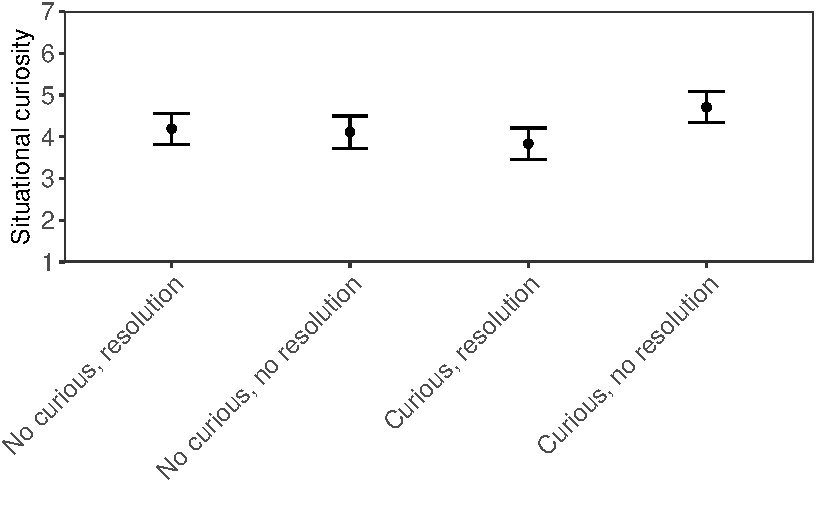
\includegraphics{curiosity_student-pilot_data-analysis_files/figure-pdf/fig-asitcur-1.pdf}

}

\caption{\label{fig-asitcur}Mean of situational curiosity by
experimental condition for the astronomy issue.}

\end{figure}

\begin{figure}

{\centering 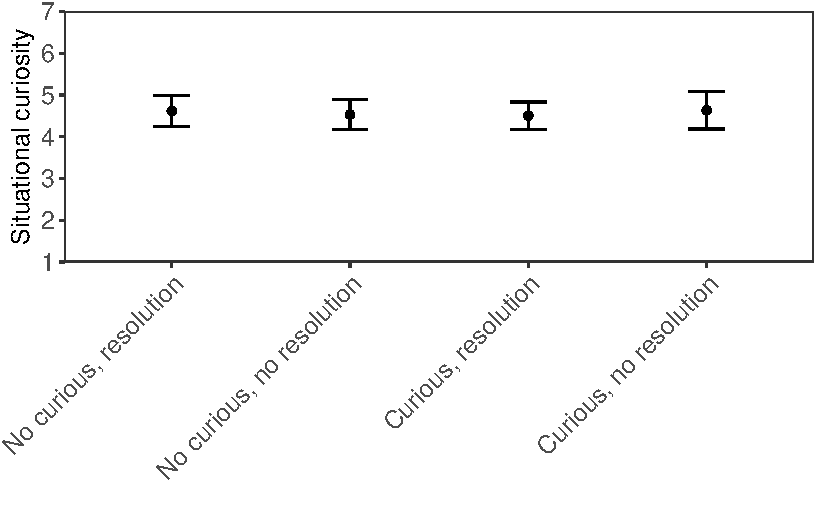
\includegraphics{curiosity_student-pilot_data-analysis_files/figure-pdf/fig-rsitcur-1.pdf}

}

\caption{\label{fig-rsitcur}Mean of situational curiosity by
experimental condition for the rain/geosmin issue.}

\end{figure}

\begin{figure}

{\centering 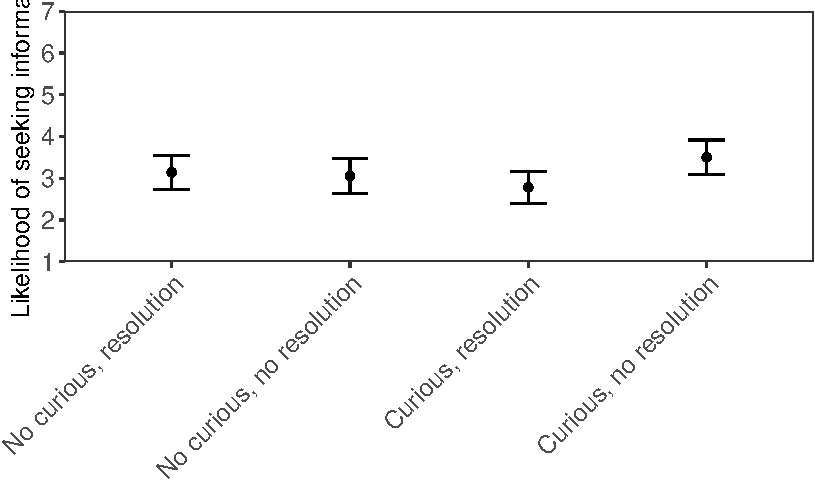
\includegraphics{curiosity_student-pilot_data-analysis_files/figure-pdf/fig-ainfoseek-1.pdf}

}

\caption{\label{fig-ainfoseek}Mean of information seeking by
experimental condition for the astronomy issue.}

\end{figure}

\begin{figure}

{\centering 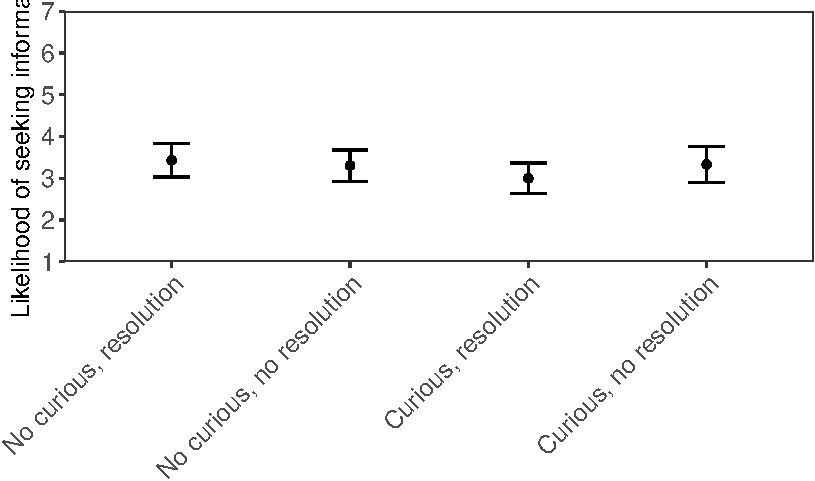
\includegraphics{curiosity_student-pilot_data-analysis_files/figure-pdf/fig-rinfoseek-1.pdf}

}

\caption{\label{fig-rinfoseek}Mean of information seeking by
experimental condition for the rain/geosmin issue.}

\end{figure}

\begin{figure}

{\centering 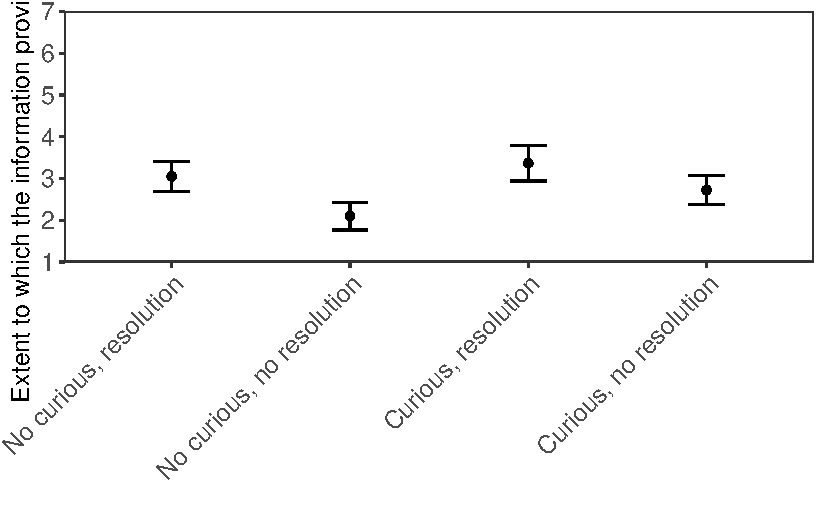
\includegraphics{curiosity_student-pilot_data-analysis_files/figure-pdf/fig-aclosure-1.pdf}

}

\caption{\label{fig-aclosure}Mean of index tapping the extent to which
the information provided closure by experimental condition for the
astronomy issue.}

\end{figure}

\begin{figure}

{\centering 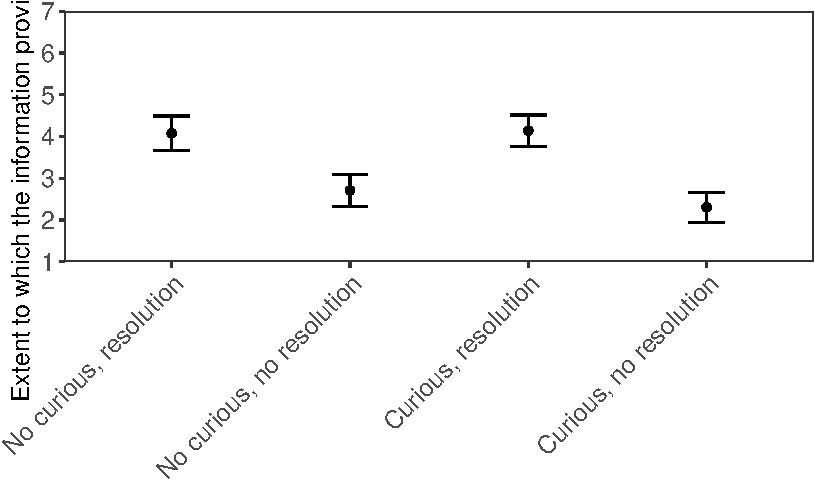
\includegraphics{curiosity_student-pilot_data-analysis_files/figure-pdf/fig-rclosure-1.pdf}

}

\caption{\label{fig-rclosure}Mean of index tapping the extent to which
the information provided closure by experimental condition for the
rain/geosmin issue.}

\end{figure}

\hypertarget{tbl-asitcur}{}
\begin{table}[!h]
\caption{\label{tbl-asitcur}OLS regression predicting situational curiosity for the astronomy
conditions. }\tabularnewline

\centering
\begin{tabular}{lr}
\toprule
\cellcolor{gray!10}{Observations} & \cellcolor{gray!10}{235}\\
Dependent variable & asitcur\\
\cellcolor{gray!10}{Type} & \cellcolor{gray!10}{OLS linear regression}\\
\bottomrule
\end{tabular}
\end{table} \begin{table}[!h]
\centering
\begin{tabular}{lr}
\toprule
\cellcolor{gray!10}{F(2,232)} & \cellcolor{gray!10}{1.91}\\
R² & 0.02\\
\cellcolor{gray!10}{Adj. R²} & \cellcolor{gray!10}{0.01}\\
\bottomrule
\end{tabular}
\end{table} \begin{table}[!h]
\centering
\begin{threeparttable}
\begin{tabular}{lrrrr}
\toprule
  & Est. & S.E. & t val. & p\\
\midrule
\cellcolor{gray!10}{(Intercept)} & \cellcolor{gray!10}{4.36} & \cellcolor{gray!10}{0.17} & \cellcolor{gray!10}{26.37} & \cellcolor{gray!10}{0.00}\\
acuriousCurious & 0.09 & 0.19 & 0.45 & 0.65\\
\cellcolor{gray!10}{aresoResolution} & \cellcolor{gray!10}{-0.37} & \cellcolor{gray!10}{0.19} & \cellcolor{gray!10}{-1.91} & \cellcolor{gray!10}{0.06}\\
\bottomrule
\end{tabular}
\begin{tablenotes}
\item Standard errors: OLS
\end{tablenotes}
\end{threeparttable}
\end{table}

\hypertarget{tbl-rsitcur}{}
\begin{table}[!h]
\caption{\label{tbl-rsitcur}OLS regression predicting situational curiosity for the rain/geosmin
conditions. }\tabularnewline

\centering
\begin{tabular}{lr}
\toprule
\cellcolor{gray!10}{Observations} & \cellcolor{gray!10}{237}\\
Dependent variable & rsitcur\\
\cellcolor{gray!10}{Type} & \cellcolor{gray!10}{OLS linear regression}\\
\bottomrule
\end{tabular}
\end{table} \begin{table}[!h]
\centering
\begin{tabular}{lr}
\toprule
\cellcolor{gray!10}{F(2,234)} & \cellcolor{gray!10}{0.06}\\
R² & 0.00\\
\cellcolor{gray!10}{Adj. R²} & \cellcolor{gray!10}{-0.01}\\
\bottomrule
\end{tabular}
\end{table} \begin{table}[!h]
\centering
\begin{threeparttable}
\begin{tabular}{lrrrr}
\toprule
  & Est. & S.E. & t val. & p\\
\midrule
\cellcolor{gray!10}{(Intercept)} & \cellcolor{gray!10}{4.60} & \cellcolor{gray!10}{0.16} & \cellcolor{gray!10}{28.21} & \cellcolor{gray!10}{0.00}\\
rcuriousCurious & -0.06 & 0.19 & -0.34 & 0.73\\
\cellcolor{gray!10}{rresoResolution} & \cellcolor{gray!10}{-0.01} & \cellcolor{gray!10}{0.19} & \cellcolor{gray!10}{-0.07} & \cellcolor{gray!10}{0.95}\\
\bottomrule
\end{tabular}
\begin{tablenotes}
\item Standard errors: OLS
\end{tablenotes}
\end{threeparttable}
\end{table}

\hypertarget{tbl-ainfoseek}{}
\begin{table}[!h]
\caption{\label{tbl-ainfoseek}OLS regression predicting likelihood of seeking information for the
astronomy conditions. }\tabularnewline

\centering
\begin{tabular}{lr}
\toprule
\cellcolor{gray!10}{Observations} & \cellcolor{gray!10}{235}\\
Dependent variable & ainfoseek\\
\cellcolor{gray!10}{Type} & \cellcolor{gray!10}{OLS linear regression}\\
\bottomrule
\end{tabular}
\end{table} \begin{table}[!h]
\centering
\begin{tabular}{lr}
\toprule
\cellcolor{gray!10}{F(2,232)} & \cellcolor{gray!10}{1.31}\\
R² & 0.01\\
\cellcolor{gray!10}{Adj. R²} & \cellcolor{gray!10}{0.00}\\
\bottomrule
\end{tabular}
\end{table} \begin{table}[!h]
\centering
\begin{threeparttable}
\begin{tabular}{lrrrr}
\toprule
  & Est. & S.E. & t val. & p\\
\midrule
\cellcolor{gray!10}{(Intercept)} & \cellcolor{gray!10}{3.24} & \cellcolor{gray!10}{0.18} & \cellcolor{gray!10}{18.33} & \cellcolor{gray!10}{0.00}\\
acuriousCurious & 0.06 & 0.21 & 0.28 & 0.78\\
\cellcolor{gray!10}{aresoResolution} & \cellcolor{gray!10}{-0.33} & \cellcolor{gray!10}{0.21} & \cellcolor{gray!10}{-1.60} & \cellcolor{gray!10}{0.11}\\
\bottomrule
\end{tabular}
\begin{tablenotes}
\item Standard errors: OLS
\end{tablenotes}
\end{threeparttable}
\end{table}

\hypertarget{tbl-rinfoseek}{}
\begin{table}[!h]
\caption{\label{tbl-rinfoseek}OLS regression predicting likelihood of seeking information for the
rain/geosmin conditions. }\tabularnewline

\centering
\begin{tabular}{lr}
\toprule
\cellcolor{gray!10}{Observations} & \cellcolor{gray!10}{237}\\
Dependent variable & rinfoseek\\
\cellcolor{gray!10}{Type} & \cellcolor{gray!10}{OLS linear regression}\\
\bottomrule
\end{tabular}
\end{table} \begin{table}[!h]
\centering
\begin{tabular}{lr}
\toprule
\cellcolor{gray!10}{F(2,234)} & \cellcolor{gray!10}{0.73}\\
R² & 0.01\\
\cellcolor{gray!10}{Adj. R²} & \cellcolor{gray!10}{-0.00}\\
\bottomrule
\end{tabular}
\end{table} \begin{table}[!h]
\centering
\begin{threeparttable}
\begin{tabular}{lrrrr}
\toprule
  & Est. & S.E. & t val. & p\\
\midrule
\cellcolor{gray!10}{(Intercept)} & \cellcolor{gray!10}{3.42} & \cellcolor{gray!10}{0.17} & \cellcolor{gray!10}{20.01} & \cellcolor{gray!10}{0.00}\\
rcuriousCurious & -0.22 & 0.20 & -1.09 & 0.28\\
\cellcolor{gray!10}{rresoResolution} & \cellcolor{gray!10}{-0.10} & \cellcolor{gray!10}{0.20} & \cellcolor{gray!10}{-0.48} & \cellcolor{gray!10}{0.63}\\
\bottomrule
\end{tabular}
\begin{tablenotes}
\item Standard errors: OLS
\end{tablenotes}
\end{threeparttable}
\end{table}

\hypertarget{tbl-aclosure}{}
\begin{table}[!h]
\caption{\label{tbl-aclosure}OLS regression predicting the extent to which the information provided
closure for participants in the astronomy conditions. }\tabularnewline

\centering
\begin{tabular}{lr}
\toprule
\cellcolor{gray!10}{Observations} & \cellcolor{gray!10}{235}\\
Dependent variable & aclosure\\
\cellcolor{gray!10}{Type} & \cellcolor{gray!10}{OLS linear regression}\\
\bottomrule
\end{tabular}
\end{table} \begin{table}[!h]
\centering
\begin{tabular}{lr}
\toprule
\cellcolor{gray!10}{F(2,232)} & \cellcolor{gray!10}{12.58}\\
R² & 0.10\\
\cellcolor{gray!10}{Adj. R²} & \cellcolor{gray!10}{0.09}\\
\bottomrule
\end{tabular}
\end{table} \begin{table}[!h]
\centering
\begin{threeparttable}
\begin{tabular}{lrrrr}
\toprule
  & Est. & S.E. & t val. & p\\
\midrule
\cellcolor{gray!10}{(Intercept)} & \cellcolor{gray!10}{2.17} & \cellcolor{gray!10}{0.16} & \cellcolor{gray!10}{13.52} & \cellcolor{gray!10}{0.00}\\
acuriousCurious & 0.47 & 0.19 & 2.50 & 0.01\\
\cellcolor{gray!10}{aresoResolution} & \cellcolor{gray!10}{0.80} & \cellcolor{gray!10}{0.19} & \cellcolor{gray!10}{4.27} & \cellcolor{gray!10}{0.00}\\
\bottomrule
\end{tabular}
\begin{tablenotes}
\item Standard errors: OLS
\end{tablenotes}
\end{threeparttable}
\end{table}

\hypertarget{tbl-rclosure}{}
\begin{table}[!h]
\caption{\label{tbl-rclosure}OLS regression predicting the extent to which the information provided
closure for participants in the rain/geosmin conditions. }\tabularnewline

\centering
\begin{tabular}{lr}
\toprule
\cellcolor{gray!10}{Observations} & \cellcolor{gray!10}{237}\\
Dependent variable & rclosure\\
\cellcolor{gray!10}{Type} & \cellcolor{gray!10}{OLS linear regression}\\
\bottomrule
\end{tabular}
\end{table} \begin{table}[!h]
\centering
\begin{tabular}{lr}
\toprule
\cellcolor{gray!10}{F(2,234)} & \cellcolor{gray!10}{35.86}\\
R² & 0.23\\
\cellcolor{gray!10}{Adj. R²} & \cellcolor{gray!10}{0.23}\\
\bottomrule
\end{tabular}
\end{table} \begin{table}[!h]
\centering
\begin{threeparttable}
\begin{tabular}{lrrrr}
\toprule
  & Est. & S.E. & t val. & p\\
\midrule
\cellcolor{gray!10}{(Intercept)} & \cellcolor{gray!10}{2.58} & \cellcolor{gray!10}{0.17} & \cellcolor{gray!10}{15.47} & \cellcolor{gray!10}{0.00}\\
rcuriousCurious & -0.20 & 0.19 & -1.04 & 0.30\\
\cellcolor{gray!10}{rresoResolution} & \cellcolor{gray!10}{1.62} & \cellcolor{gray!10}{0.19} & \cellcolor{gray!10}{8.42} & \cellcolor{gray!10}{0.00}\\
\bottomrule
\end{tabular}
\begin{tablenotes}
\item Standard errors: OLS
\end{tablenotes}
\end{threeparttable}
\end{table}



\end{document}
